%!TEX root = spire-project.tex

\subsubsection{Calibration of spatial frequency axis}

To determine which values of spatial frequency correspond to pixel distances of the image in the Fourier space one can use a Gaussian image. A Gaussian has the advantage that the Fouier transfrom is also a Gaussian.

\begin{equation}
    f(x) \propto e^{\frac{-x^2}{2\sigma^2}}
    \label{gauss}
\end{equation}

\begin{equation}
    \mathscr{F}(f) \propto e^{-\frac{\sigma^2\omega^2}{2}}
    \label{fgauss}
\end{equation}

Disregarding amplitude, as only the width is cared about, equation \ref{gauss} shows the Gaussian function with a width paramter $\sigma$ and position $x$, and equation \ref{fgauss} shows the Fourier transform of the same gaussian in frequency space $\omega$ \citep{ozaktas2001fractional}. By fitting a guassian to the output spectra then it is possible to determine the relationship between pixel width and inverse angular distance.

\subsubsection{Determining resolution from Power Spectra}

\begin{figure*}
    \centering
    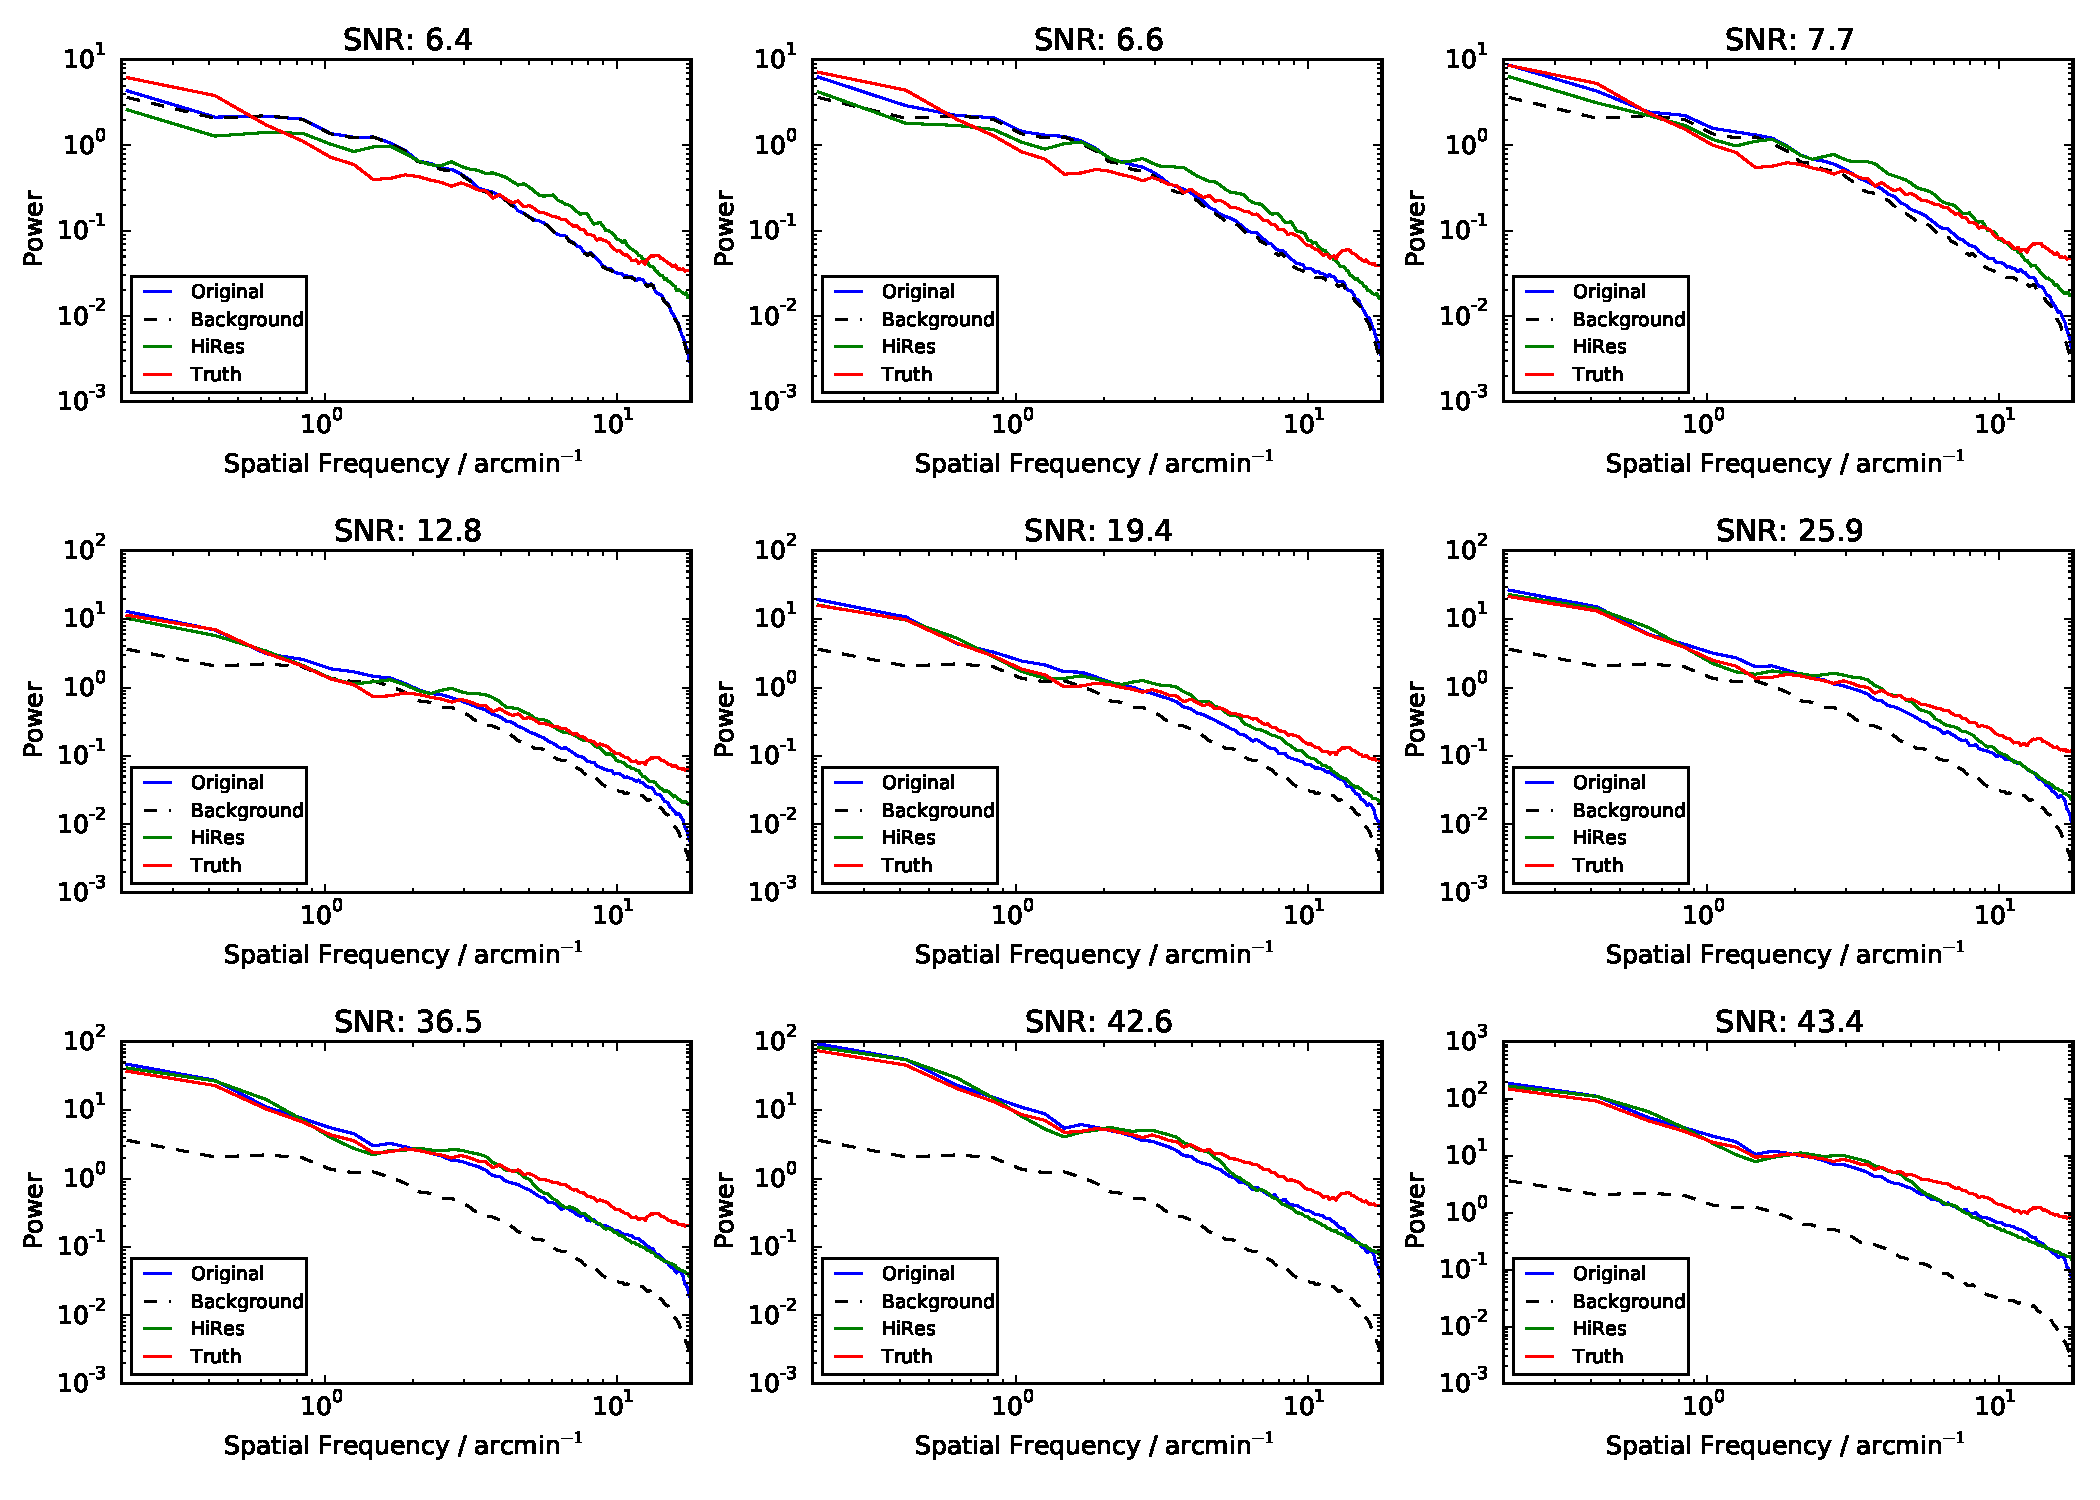
\includegraphics[width=0.9\linewidth]{figures/power-spectra.pdf}
    \caption[Power Spectra]{Power Spectra for a selection of SNR simulations}
    \label{pspectra}
\end{figure*}

When a Fourier transform of an image set is generated by the computer, a power spectrum is also produced. This roughly shows how much information there is in the waves that make up the Fourier transform.

By looking at the power spectra of the simulated image, and comparing this to the power spectra for both the HiRes output and the truth image it was hoped that information about the angular resolution improvement of HiRes could be obtained. In theory there should be a drop in the power spectrum at the point at which no more higher resolution information exists in the image.

\begin{figure}[H]
    \centering
    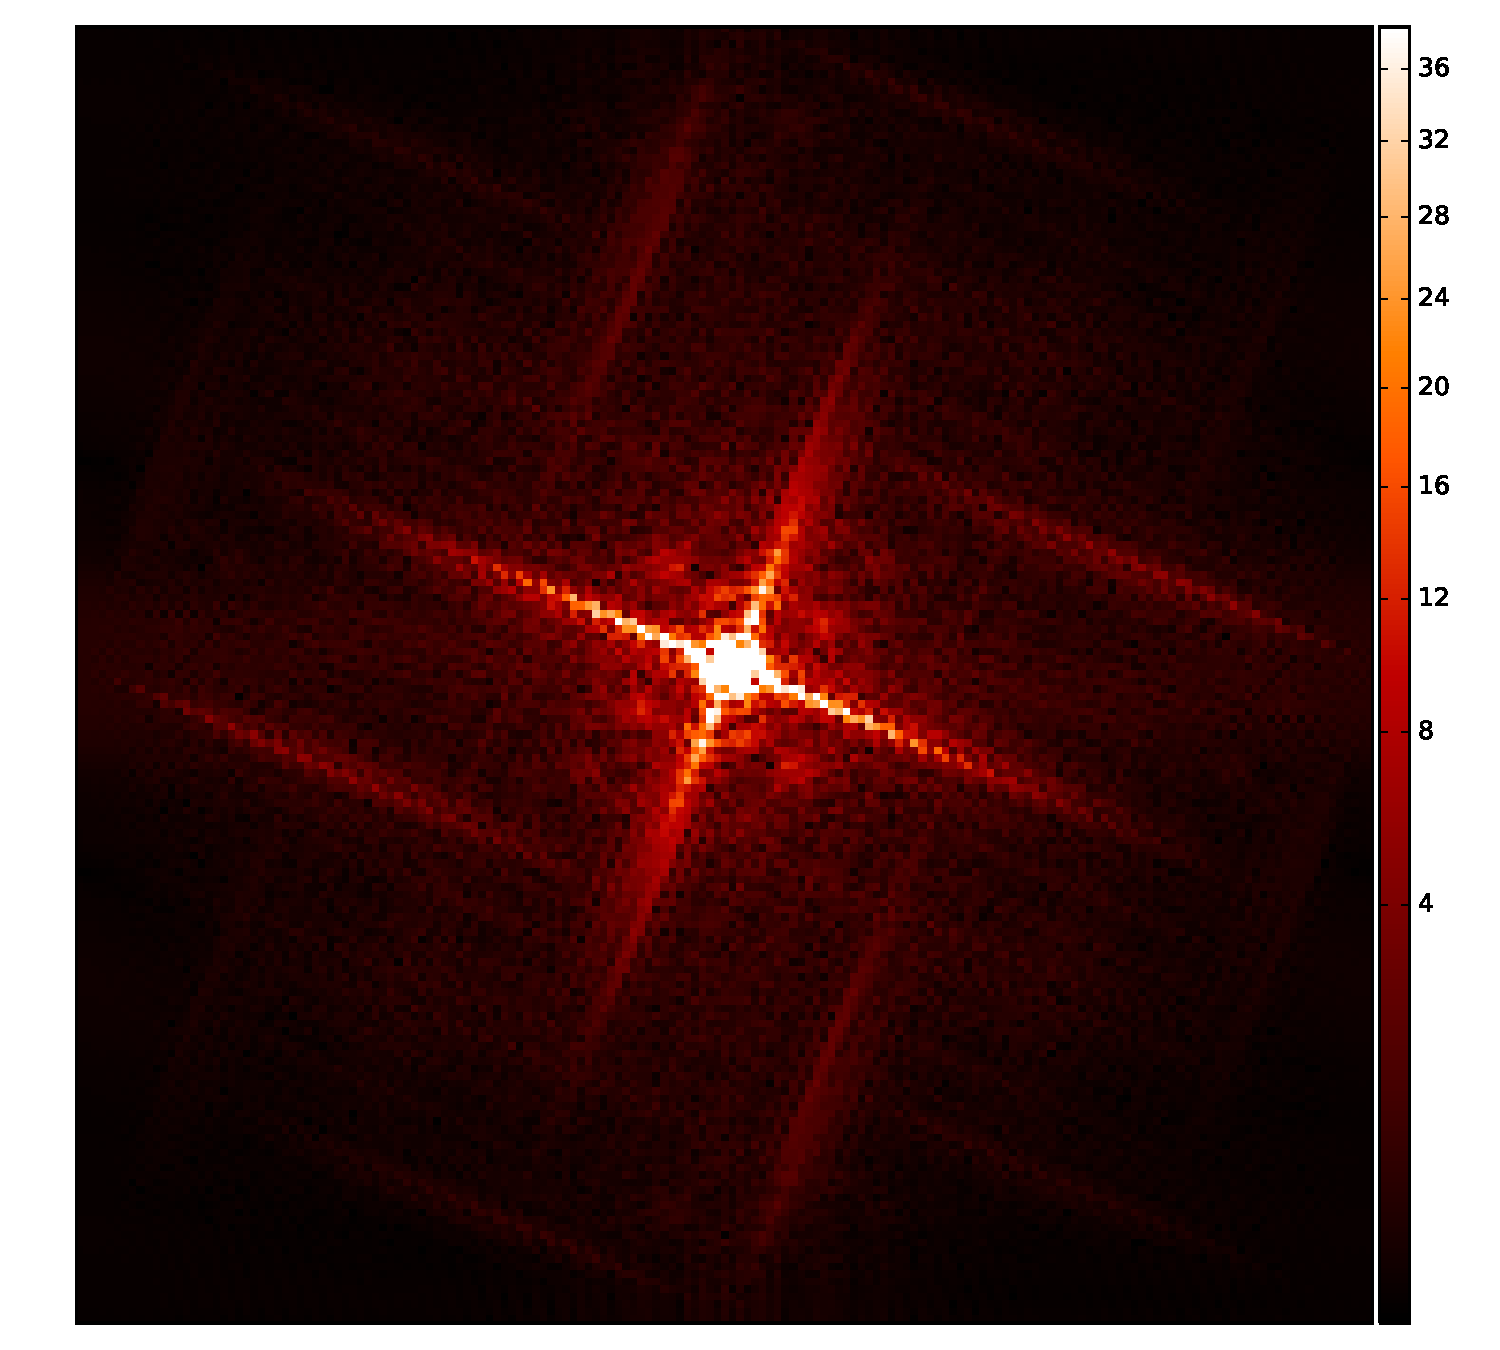
\includegraphics[width=0.8\linewidth]{figures/power-spec-sample.pdf}
    \caption[Example Power Spectrum]{Example of a generated power spectrum of an M74 observation}
    \label{spec-sample}
\end{figure}

The power spectra returned from the HIPE software routines however do not return data as typically expected. Instead of the using the central pixel as the lowest frequency wave, the returned power spectra instead is split into 4 regions, where the corner pixels of the image instead are used to indicate the lowest frequency. These spectra then need to be fixed before being used for analysis. This was done by rearranging the data such that the returned spectrum appears as expected, an example of which is shown in Figure \ref{spec-sample}. This figure is plotted with a square root normalisation as a power spectra is a square of the flux. This normalisation is shown in equation \ref{spec-scale}, where $I$ is the displayed value, $x$ is the value in the power spectrum, and $v_{min}$ and $v_{max}$ are the minimum and maximum values in the spectrum.

\begin{equation}
    I = \sqrt{\frac{x - v_{min}}{v_{max}-v_{min}}}
    \label{spec-scale}
\end{equation}

 To convert this into the graphs as seen in Figure \ref{pspectra} it is necessary to average the data at radial intervals. While this can be done by taking radial apertures and averaging the pixel values within, I decided to follow a simpler strategy that wont have any overlapping or missing pixels, or have to allow for apertures partially containing pixels. I process each of the power spectra by iterating over each pixel index, and building a histogram of the average pixel values in single pixel radial bins. This gives the 1D power spectra as shown in Figure \ref{pspectra}.

In practice however this can be very difficult to disentangle from the noise in the spectra, and I was unable to obtain any useful information from the power spectra, a sample of which is shown in figure \ref{pspectra}. It was a shame that this produced no useable information as the implementation of this part of the project took up a significant portion of the time. It is possible that further analysis of this, and performing the same analysis of different observations may allow some useful data to be obtained from this method.
